
\chapter{Decimals}
\section{Introduction to Decimals}
\thispagestyle{fancy}

We use decimals every day as we buy things. For example, each pound of apple costs \$$1.99$. In this lesson, we will learn the definition of decimals.

\subsection{Definition of Decimals}
The best way to understand decimals is to think of money, because we deal with money every day. For example, $1.99$ means $1$ dollar and $99$ cents.

\subsection{Types of Decimals}
There are a few types of decimals:
\begin{itemize}
\item \textbf{terminating decimal}: A terminating decimal has a limited number of places, like $0.1,1.23,1.2345$.
\item \textbf{repeating decimal}: A repeating decimal goes on forever repeating the same digits again and again, like $0.111...,4.121212...,5.3124124124...$. A repeating decimal can be re-written with a bar over the repeating digits:
\[
\begin{aligned}[t]
	0.111... &= 0.\overline{1} \\
	4.121212... &= 0.\overline{12} \\
	5.3124124124... &= 5.3\overline{124} 
\end{aligned}
\]
\item \textbf{irrational decimal}: An irrational decimal goes on forever without repeating any pattern. Here are a few examples:
\[
\begin{aligned}[t]
	\pi &= 3.1415926... \\
	\sqrt{2} &= 1.414... \\
	\sqrt{3} &= 1.732...
\end{aligned}
\]
\end{itemize}

\subsubsection{The decimal $0.03$}
Think of the number $0.03$, which is $3$ cents. Since each dollar has $100$ cents, $0.03$ represents $3$ out of $100$, or, in fraction, $\frac{3}{100}$. This fraction is read as "three hundredths".

This is why we call the second digit after the decimal point the \textit{hundredths place.} We could read $0.03$ either as "three hundredths," or simply "zero point zero three."

Here is one way to represent $0.03$ graphically (the grid has $100$ cells):

\begin{center}
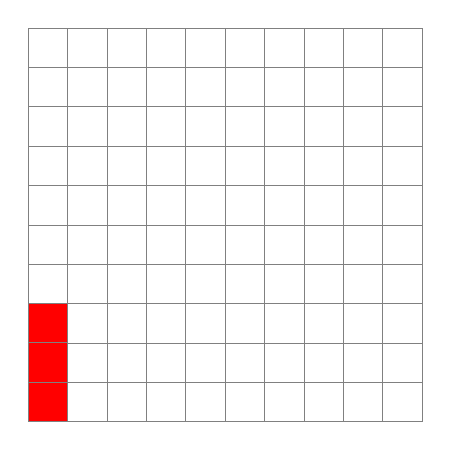
\begin{tikzpicture}
	\draw[step=0.5cm,gray,very thin] (0,0) grid (5,5);
	\filldraw[fill=red, draw=gray] (0,0) rectangle (0.5,0.5);
	\filldraw[fill=red, draw=gray] (0,0.5) rectangle (0.5,1);
	\filldraw[fill=red, draw=gray] (0,1) rectangle (0.5,1.5);
\end{tikzpicture}
\captionof{figure}{Graphic representation of $0.03$}
\end{center}

\subsubsection{The decimal $0.3$}
Let's look at another number: $0.3$. This number does not represent $3$ cents, because earlier we learned $0.03$ represents $3$ cents. The difference is that, in $0.3$, the number $3$ is in the tenths place. In terms of money, $0.3$ represents $30$ cents. On a price mark, we usually write $0.3$ as \$$0.30$. This revealed an important property of decimals:

\textbf{If we add the digit $0$ to the end of a decimal (behind the decimal point), the decimal's value doesn't change.} For example: $0.30=0.3$, $0.300=0.3$, $1.20=1.2$.

Note that $1.3\neq1.03$: the number $1.3$ represents a dollar and $30$ cents, while the number $1.03$ represents a dollar and $3$ cents.

The number $0.3$ represents $3$ out of $10$, or, in fraction, $\frac{3}{10}$. This fraction is read as "three tenths".

This is why we call the digit after the decimal point the \textit{tenths place.} We could read $0.3$ either as "three tenths," or simply "zero point three."

Here is one way to represent $0.3$ graphically:

\begin{center}
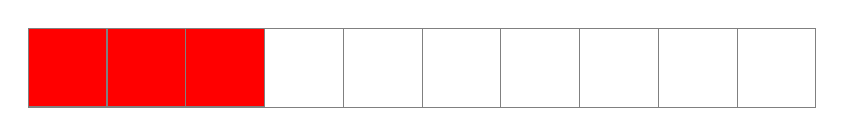
\begin{tikzpicture}
	\draw[step=1cm,gray,very thin] (0,0) grid (10,1);
	\filldraw[fill=red, draw=gray] (0,0) rectangle (1,1);
	\filldraw[fill=red, draw=gray] (1,0) rectangle (2,1);
	\filldraw[fill=red, draw=gray] (2,0) rectangle (3,1);
\end{tikzpicture}
\captionof{figure}{Graphic representation of $0.3$}
\end{center}

\subsubsection{The decimal $0.003$}
Finally, let's look at $0.003$. Earlier, we learned that $0.03$ represents $3$ cents. The number $0.003$ is three tenth of a cent. If you look carefully at gas price next time you fill up, each gallon actually costs something like \$$3.159$. Notice the last digit is always $9$. Nine tenths of a cent is not a lot of money, but the profit adds up.

The number $0.003$ represents $3$ out of $1000$, or, in fraction, $\frac{3}{1000}$. This fraction is read as "three thousandths".

This is why we call the third digit after the decimal point the \textit{thousandths place.} We could read $0.003$ either as "three thousandths," or simply "zero point zero zero three."

We will not represent $0.003$ graphically here, because it's hard to draw a grid with $1,000$ cells.

\subsection{Read Decimals}
For the decimal $1,234.5678$, here are the names of each digit:
\begin{itemize}
\item $1$ is in the thousands place, representing one thousand.
\item $2$ is in the hundreds place, representing two hundred.
\item $3$ is in the tens place, representing thirty.
\item $4$ is in the ones place, representing four.
\item $5$ is in the tenths place, representing five tenths ($50$ cents).
\item $6$ is in the hundredths place, representing six hundredths ($6$ cents).
\item $7$ is in the thousandths place, representing seven thousandths.
\item $8$ is in the ten-thousandths place, representing eight ten-thousandths.
\end{itemize}

Here are a few examples of how to read decimals:

\begin{itemize}
\item $12.3$ reads: twelve and three tenths
\item $12.34$ reads: twelve and thirty four hundredths
\item $12.345$ reads: twelve and three hundred forty-five thousandths
\item $12.3456$ reads: twelve and three thousand four hundred fifty-six ten-thousandths
\item $12.03$ reads: twelve and three hundredths
\item $12.003$ reads: twelve and three thousandths
\end{itemize}

\subsection{Decimals on Number Line}
Here are a few examples on how to locate decimals on the number line:

\begin{center} 
\begin{tikzpicture}
% a straight line segment
\draw [<->] (0,0) -- (12,0);
% the ticks and their labels
\foreach \x  in {1,...,11}
  \draw[xshift=\x cm] (0pt,2pt) -- (0pt,-1pt);
\node[fill=black,draw=black,circle,inner sep=2pt,label=below:{$0$}] at (1,0) {};
\node[fill=black,draw=black,circle,inner sep=2pt,label=below:{$1$}] at (11,0) {};
\node[fill=red,draw=red,circle,inner sep=2pt,label=above:{$0.3$}] at (4,0) {};
\end{tikzpicture}

\begin{tikzpicture}
% a straight line segment
\draw [<->] (0,0) -- (12,0);
% the ticks and their labels
\foreach \x  in {1,...,11}
  \draw[xshift=\x cm] (0pt,2pt) -- (0pt,-1pt);
\node[fill=black,draw=black,circle,inner sep=2pt,label=below:{$-3$}] at (1,0) {};
\node[fill=black,draw=black,circle,inner sep=2pt,label=below:{$-2$}] at (11,0) {};
\node[fill=red,draw=red,circle,inner sep=2pt,label=above:{$-2.7$}] at (4,0) {};
\end{tikzpicture}

\begin{tikzpicture}
% a straight line segment
\draw [<->] (0,0) -- (12,0);
% the ticks and their labels
\foreach \x  in {1,...,11}
  \draw[xshift=\x cm] (0pt,2pt) -- (0pt,-1pt);
\node[fill=black,draw=black,circle,inner sep=2pt,label=below:{$-3.1$}] at (1,0) {};
\node[fill=black,draw=black,circle,inner sep=2pt,label=below:{$-3$}] at (11,0) {};
\node[fill=red,draw=red,circle,inner sep=2pt,label=above:{$-3.07$}] at (4,0) {};
\end{tikzpicture}
\captionof{figure}{Decimals on the number line}
\end{center}

\subsection{Compare Decimals}
Which one is bigger, $3.09$ or $3.81$? It's easy to compare if we think about money: three dollars and eighty-one cents is bigger than three dollars and nine cents. So we have:
\[ 3.09<3.81 \]

So, when we compare decimals, we compare the tenths' place first, and then the hundredths' place. Even though the digit $9$ in $3.09$ is bigger than $8$ in $3.81$, the number $3.81$ is bigger than $3.09$.

We have the following comparisons:
\[
\begin{aligned}[t]
	1.29 &< 1.30 \\
	4.29 &> 1.30 \\
	3.04 &< 3.4 \\
	0.031 &> 0.009 
\end{aligned}
\]
Comparing negative numbers is "opposite:"
\[
\begin{aligned}[t]
	-1.29 &> -1.30 \\
	-4.29 &< -1.30 \\
	-3.04 &> -3.4 \\
	-0.031 &< -0.009 
\end{aligned}
\]
Finally, be careful when there are trailing zeroes:
\[
\begin{aligned}[t]
	1.10 &= 1.1 \\
	0.03 &= 0.030 \\
	-0.300 &= -0.3 
\end{aligned}
\]

\subsection{Round Decimals}
Earlier, we learned how to round whole numbers. The concept of rounding decimals is the same. For example, to round $1.19$ to an integer, we have $1.19\approx1$ because $1.19$ is closer to $1$ than $2$. Let's look at a few examples:

\begin{myexample}
Round $1.295$ to the tenths place.
\end{myexample}
\begin{solution}
In $1.295$, the tenths place is $2$. The digit behind it is $9$. Since $9$ is bigger than $4$, we round up:
\[ 1.295 \approx 1.3 \]
\end{solution}

\begin{myexample}
Round $1.245$ to the tenths place.
\end{myexample}
\begin{solution}
In $1.245$, the tenths place is $2$. The digit behind it is $4$. Since $4$ is smaller than $5$, we don't round up:
\[ 1.245 \approx 1.2 \]
\end{solution}

\begin{myexample}
Round $1.295$ to the hundredths place.
\end{myexample}
\begin{solution}
In $1.295$, the hundredths place is $9$. The digit behind it is $5$. Since $5$ is bigger than $4$, we round up:
\[ 1.295 \approx 1.30 \]
\end{solution}

